\section{Introduction}

\noindent This template provides a brief, generic introduction suitable for an EPFL School of Life Sciences master thesis. It motivates the need for clear, reproducible, and data\,driven analyses without binding the thesis to a specific application.

\noindent The following chapters outline a general methodology, present representative results, and discuss implications and limitations. Replace this placeholder with project\,specific objectives, datasets, and contributions.

\bigskip

\noindent Figure~\ref{fig:cell-overview} shows how to insert and reference a single image. In Figure~\ref{fig:cell-subfigures}, panels~\subref{fig:cell-sub-a} and~\subref{fig:cell-sub-b} demonstrate subfigures and cross\,referencing to specific panels.

\begin{figure}[h]
  \centering
  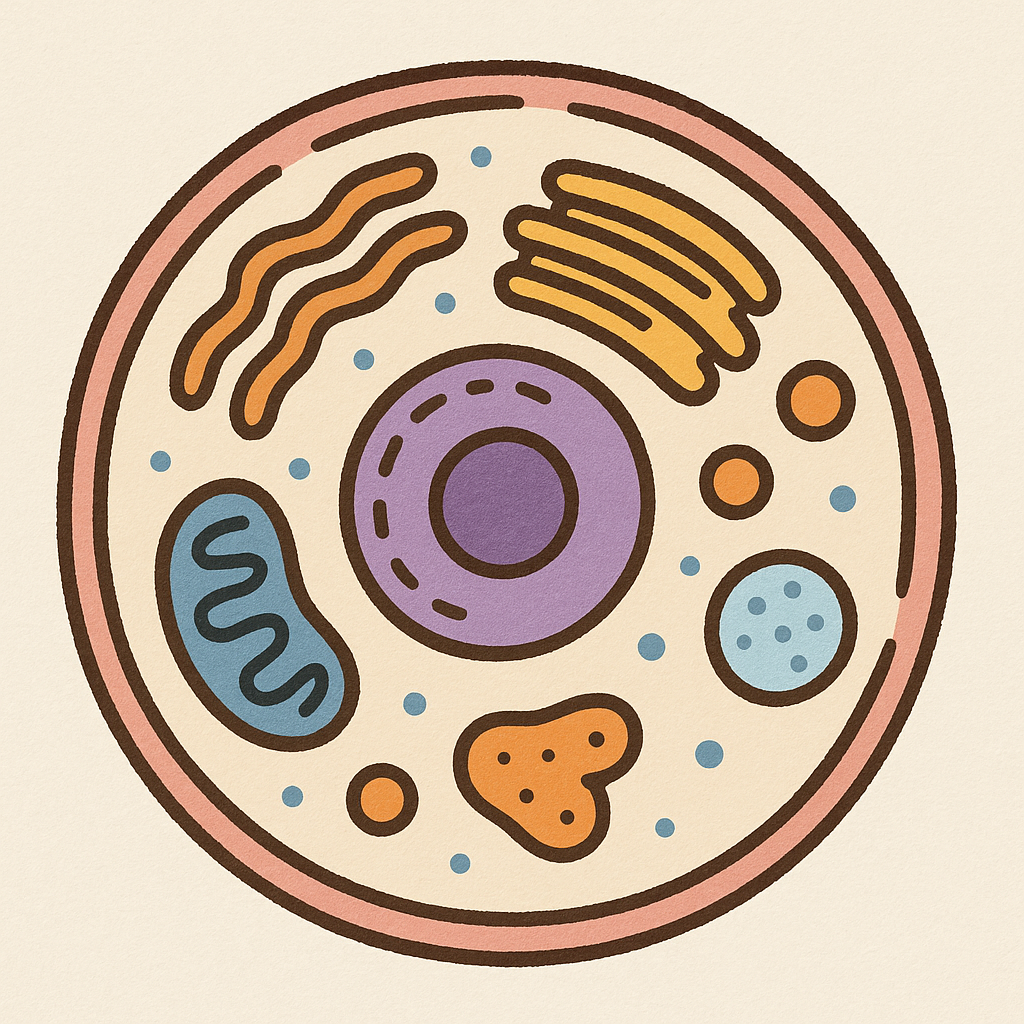
\includegraphics[width=0.48\textwidth]{figures/cell.png}
  \caption{Overview illustration: a mother cell giving rise to two daughter cells.}
  \label{fig:cell-overview}
\end{figure}

\begin{figure}[h]
  \centering
  \begin{subfigure}{0.48\textwidth}
    \centering
    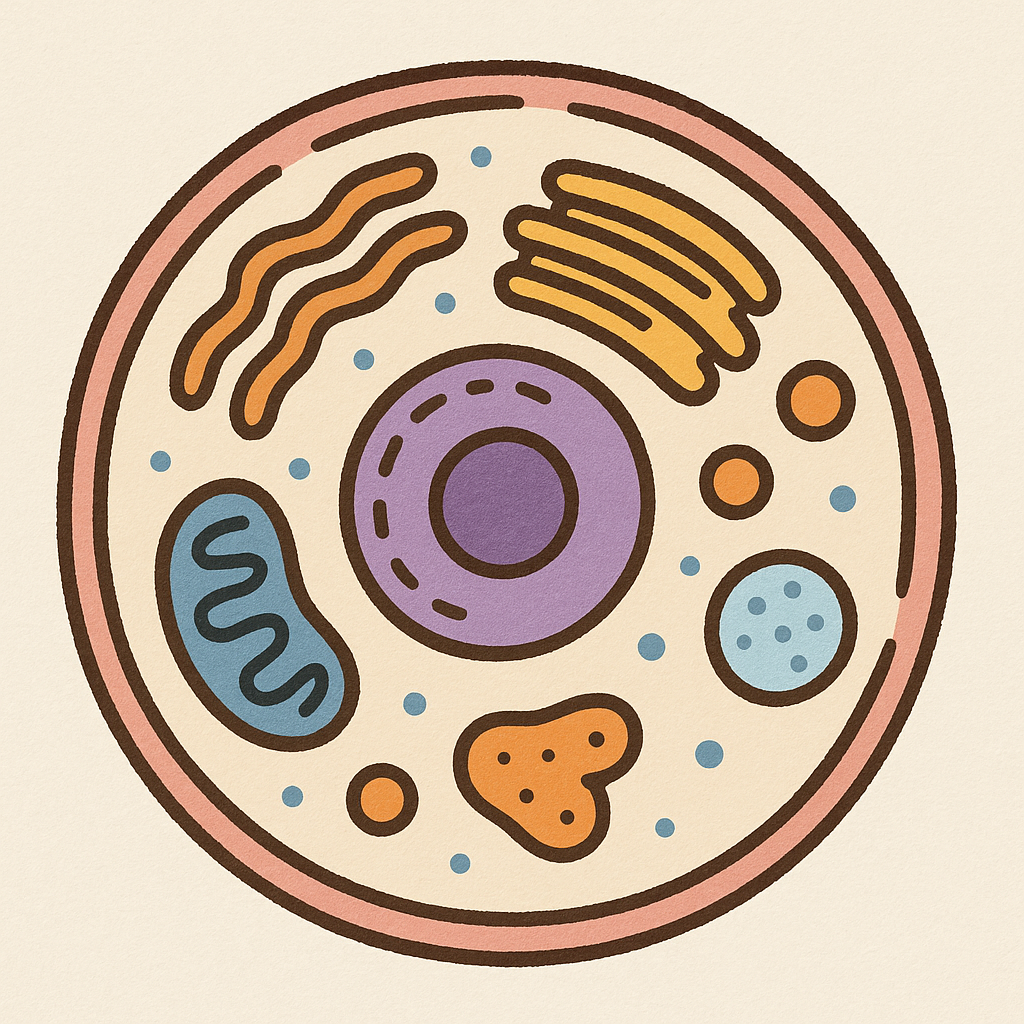
\includegraphics[width=\linewidth]{figures/cell.png}
    \caption{Daughter Cell 1.}
    \label{fig:cell-sub-a}
  \end{subfigure}\hfill
  \begin{subfigure}{0.48\textwidth}
    \centering
    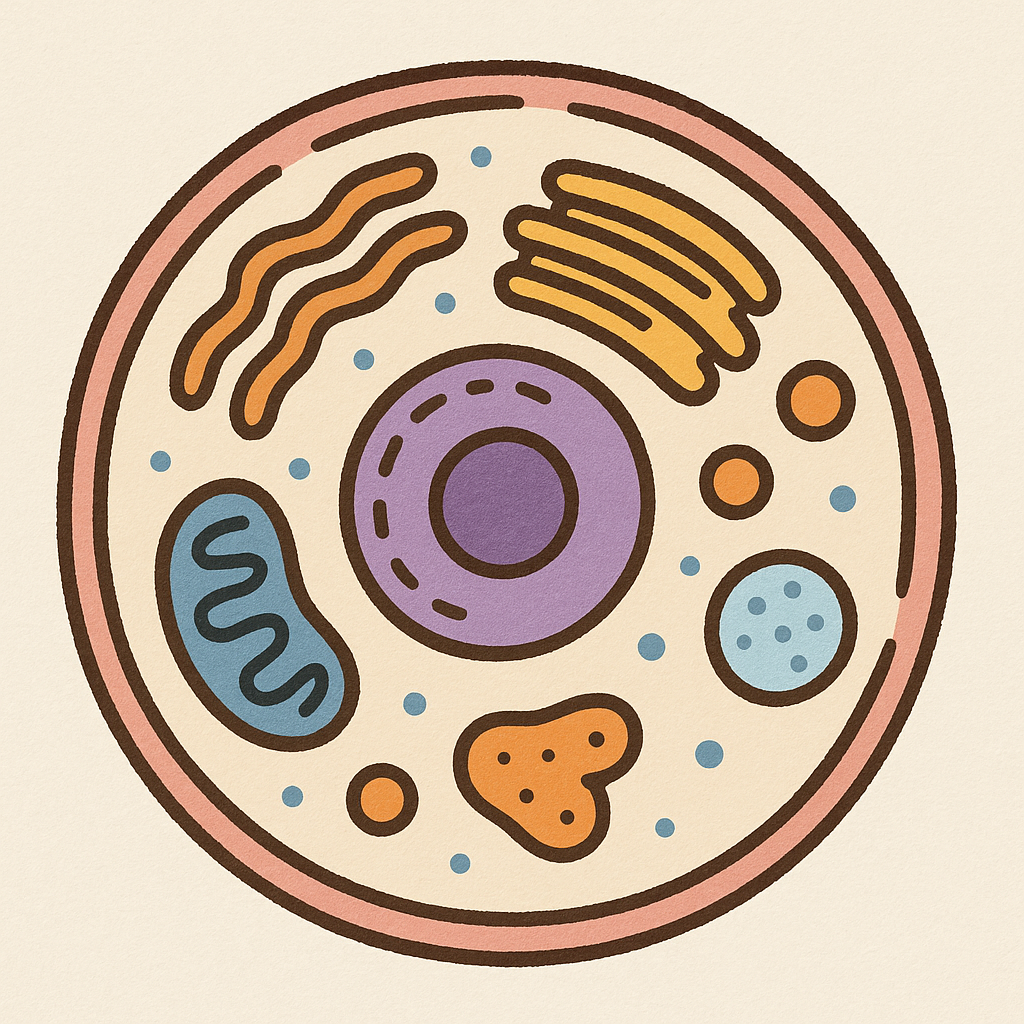
\includegraphics[width=\linewidth]{figures/cell.png}
    \caption{Daughter Cell 2.}
    \label{fig:cell-sub-b}
  \end{subfigure}
  \caption{Subfigure example: the same image reused to illustrate two conceptual panels.}
  \label{fig:cell-subfigures}
\end{figure}